\section{Fermi's golden rule}\label{sec:2.1}

A kilogram of silicon exposed for a year to \SI{100}{MeV} dark matter with $\sigmae = \SI{e-40}{cm^2}$ expects 73 events in the toy rate of \cref{we:1-limit}, and twice as many in two years: the count is a rate times an exposure (\cref{eq:1.5-Nsig}). Quantum mechanics gives probabilities, not rates. A probability that grows linearly in time appears only when a weak perturbation couples an initial state to a continuum of final states, and only within a window of times. The derivation of Fermi's golden rule follows Refs.~\cite[Chap.~5]{sakurai2017modern} and \cite[Chap.~XIII]{cohentannoudji1977quantum}.

\subsection{First-order amplitude}

The target, together with a dark-matter particle far from it, evolves under an unperturbed Hamiltonian $H_0$ with eigenstates $|n\rangle$ and energies $E_n$. At $t = 0$ a perturbation $H'(t)$ is switched on, and the system starts in the eigenstate $|i\rangle$. We expand the state in the unperturbed basis, with the free phases taken out:
\begin{equation*}
  |\psi(t)\rangle = \sum_n c_n(t)\,\ee^{-\ii E_n t}\,|n\rangle, \qquad c_n(0) = \delta_{ni}.
\end{equation*}
Inserting this into $\ii\,\partial_t|\psi\rangle = (H_0 + H')|\psi\rangle$, the time derivative of each phase cancels the action of $H_0$. Projecting onto $\ee^{-\ii E_f t}|f\rangle$ leaves an exact set of equations for the amplitudes,
\begin{equation}
  \ii\,\dot c_f(t) = \sum_n \langle f|H'(t)|n\rangle\,\ee^{\ii(E_f - E_n)t}\,c_n(t).
  \label{eq:2.1-exact}
\end{equation}
To first order in $H'$ we replace $c_n(t)$ on the right by its initial value $\delta_{ni}$ and integrate. For $f \neq i$,
\begin{equation}
  c_f(t) = -\ii\int_0^t \dd t'\,\langle f|H'(t')|i\rangle\,\ee^{\ii(E_f - E_i)t'} ,
  \label{eq:2.1-c1}
\end{equation}
and the transition probability is $P_{i\to f}(t) = |c_f(t)|^2$. The replacement is consistent only while the initial state is barely depleted, $\sum_{f\neq i}P_{i\to f}(t) \ll 1$. \Cref{eq:2.1-c1} is the first term of the Dyson series of the interaction picture; \cref{sec:2.4} takes the second.

\subsection{Constant perturbation}

Let $H'$ be independent of time for $t > 0$. This is the case of dark-matter scattering: the interaction $H_{\mathrm{int}}$ does not depend on time, and energy passes between the dark matter and the target, whose kinetic and internal energies are both in $E_i$ and $E_f$. With $\xi = E_f - E_i$ the integral in \cref{eq:2.1-c1} is elementary, $c_f(t) = -\langle f|H'|i\rangle(\ee^{\ii\xi t} - 1)/\xi$. Since $|\ee^{\ii\xi t} - 1|^2 = 2 - 2\cos\xi t = 4\sin^2(\xi t/2)$,
\begin{equation}
  P_{i\to f}(t) = 4\,|\langle f|H'|i\rangle|^2\,\frac{\sin^2(\xi t/2)}{\xi^2} .
  \label{eq:2.1-Pstatic}
\end{equation}

All the time dependence sits in the function $\sin^2(\xi t/2)/\xi^2$, drawn in \cref{fig:2-golden}(a). At $\xi = 0$ it equals $t^2/4$. Its zeros are at $\xi = 2\pi k/t$ with $k$ a nonzero integer, so the central peak has width $4\pi/t$. The substitution $u = \xi t/2$ gives its integral,
\begin{equation*}
  \int_{-\infty}^{\infty}\dd\xi\,\frac{\sin^2(\xi t/2)}{\xi^2} = \frac{t}{2}\int_{-\infty}^{\infty}\dd u\,\frac{\sin^2 u}{u^2} = \frac{\pi t}{2} ,
\end{equation*}
with $\int\dd u\,\sin^2u/u^2 = \pi$ (\cref{app:C.1}). The height grows as $t^2$, the width shrinks as $1/t$, and the area grows as $t$; the central peak holds \SI{90.3}{\percent} of it. Integrated against any function $w(\xi)$ that varies little over a range $2\pi/t$, the function returns $(\pi t/2)\,w(0)$, with a relative error $\sim 1/(t\,\Delta_{\mathrm{w}})$, where $\Delta_{\mathrm{w}}$ is the range over which $w$ varies. In the sense of distributions,
\begin{equation}
  \frac{\sin^2(\xi t/2)}{\xi^2} \;\longrightarrow\; \frac{\pi t}{2}\,\delta(\xi) \qquad (t \to \infty) ,
  \label{eq:2.1-deltalimit}
\end{equation}
which \cref{app:C.1} proves. Applied to \cref{eq:2.1-Pstatic}, it gives a probability that grows linearly in time, $P_{i\to f}(t) \to 2\pi t\,|\langle f|H'|i\rangle|^2\,\delta(E_f - E_i)$. The same limit can be taken after differentiating. The time derivative of \cref{eq:2.1-Pstatic} is $2|\langle f|H'|i\rangle|^2\sin(\xi t)/\xi$, a function of $\xi$ whose area is $\pi$ at every $t > 0$ and whose width shrinks as $1/t$; it tends to $\pi\delta(\xi)$. Since the area stays fixed while the width shrinks, the probability per unit time stops depending on $t$, and that is what we mean by a rate. The transition rate is
\begin{keyresult}[Fermi's golden rule]
\begin{equation}
  \varGamma_{i\to f} = 2\pi\,|\langle f|H'|i\rangle|^2\,\delta(E_f - E_i) .
  \label{eq:2.1-golden}
\end{equation}
The rate is defined only after summation over a continuum of final states $f$, for times in the window of \cref{eq:2.1-window}.
\end{keyresult}
In natural units the rate is an energy: $|\langle f|H'|i\rangle|^2$ carries $\mathrm{eV}^2$ and the delta function $\mathrm{eV}^{-1}$. Dividing by $\hbar$ converts it to a frequency: a rate of \SI{10}{meV} is $\SI{1.52e13}{s^{-1}}$. The delta function is energy conservation, enforced to within about $2\pi/t$ after a time $t$. For a dark-matter particle it becomes $\delta(\omega - \omega_{\vect q})$ of \cref{sec:1.3} once the dark-matter part of $E_f - E_i$ is written out (\cref{sec:2.2}).

The sudden switch-on at $t = 0$ adds a transient but does not change the rate. A perturbation turned on smoothly over a time $\tau_{\mathrm{s}}$ replaces $\sin^2(\xi t/2)/\xi^2$ by a function whose tails fall off faster in $\xi$. Its area still grows as $\pi t/2$ once $t \gg \tau_{\mathrm{s}}$, because the area counts only the time during which the perturbation acts at full strength.

\begin{figure}[tbp]
  \centering
  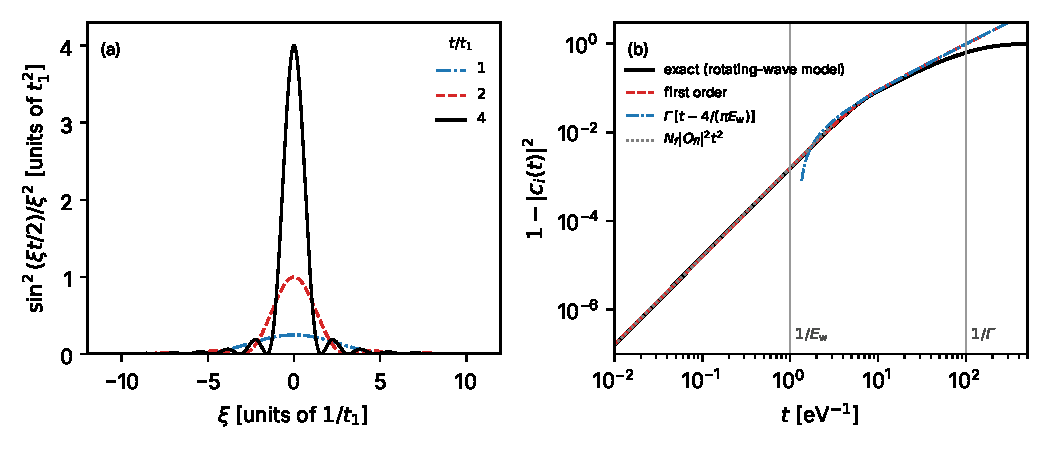
\includegraphics[width=\linewidth]{figures/ch02/fig2_1.pdf}
  \caption{(a) The function $\sin^2(\xi t/2)/\xi^2$ of the first-order transition probability, \cref{eq:2.1-Pstatic}, against the energy mismatch $\xi = E_f - E_i$, for times $t = t_1$, $2t_1$ and $4t_1$, where $t_1$ is an arbitrary unit of time ($\hbar = 1$). The peak height grows as $t^2$, the width as $1/t$, and the area, $\pi t/2$, as $t$. (b) Depletion $1 - |c_i(t)|^2$ of a discrete state coupled to a flat continuum by the absorption term of a harmonic perturbation, for the model of \cref{we:2-continuum}. It has 2000 final states spread uniformly over a width $E_{\mathrm{w}} = \SI{1}{eV}$ centered on resonance, all with the same matrix element, chosen so that the golden-rule rate is $\varGamma = \SI{10}{meV}$. Solid: exact solution of this model with the counter-rotating (emission) term dropped, by diagonalization of the 2001-level Hamiltonian in the frame rotating with the perturbation. Dashed: first-order probability, \cref{eq:2.1-WEP}. Dash-dotted: its linear long-time form. Dotted: its quadratic short-time form. Vertical lines mark $t = 1/E_{\mathrm{w}}$ (\SI{0.66}{fs}) and $t = 1/\varGamma$ (\SI{66}{fs}).}
  \label{fig:2-golden}
\end{figure}

\subsection{Conditions for a rate}

For a single discrete final state, however, \cref{eq:2.1-Pstatic} does not grow linearly. Off resonance it oscillates below $4|\langle f|H'|i\rangle|^2/\xi^2$; exactly on resonance it grows as $t^2$ until first order fails. A rate requires a continuum. Let $\mathcal{D}_f(E)\,\dd E$ be the number of final states with energies in $[E, E + \dd E]$, the \emph{density of final states}, and let $\overline{|\langle f|H'|i\rangle|^2}(E)$ be the average of the squared matrix element over those states. The total transition probability is then
\begin{equation*}
  \sum_f P_{i\to f}(t) = \int\dd E\,\mathcal{D}_f(E)\;\overline{|\langle f|H'|i\rangle|^2}(E)\;\frac{4\sin^2[(E - E_i)t/2]}{(E - E_i)^2} .
\end{equation*}
By \cref{eq:2.1-deltalimit} it becomes $\varGamma_i t$, with the total rate
\begin{equation}
  \varGamma_i = 2\pi\,\overline{|\langle f|H'|i\rangle|^2}(E_i)\;\mathcal{D}_f(E_i) .
  \label{eq:2.1-total}
\end{equation}
The catch is that $t$ has to sit in a window. Let $E_{\mathrm{w}}$ be the energy scale over which the product $\mathcal{D}_f\,\overline{|\langle f|H'|i\rangle|^2}$ changes appreciably: the width of the continuum, or of a structure within it. The delta-function limit needs the peak to be narrow on that scale, $t \gg 1/E_{\mathrm{w}}$. The sum over discrete levels becomes an integral only when the peak covers many levels, whose spacing is $1/\mathcal{D}_f$; this requires $t \ll 2\pi\mathcal{D}_f$. First-order perturbation theory requires $\varGamma_i t \ll 1$. Together,
\begin{equation}
  \frac{1}{E_{\mathrm{w}}} \ll t \ll \min\!\left(\frac{1}{\varGamma_i},\; 2\pi\mathcal{D}_f\right).
  \label{eq:2.1-window}
\end{equation}
In dark-matter scattering, however, the continuum is always present, even when the target has discrete levels, such as an atom below its ionization threshold. The final state contains the scattered dark-matter particle, whose momentum ranges over a continuum, and $\mathcal{D}_f$ counts target levels and dark-matter momenta together. Energy conservation then selects, for each target level, a shell of outgoing momenta, and the delta function of \cref{eq:2.1-golden} is integrated over that shell rather than over the target spectrum (\cref{sec:2.2}).

The upper bound $2\pi\mathcal{D}_f$ grows with the volume of the system, because $\mathcal{D}_f$ does (\cref{eq:2.1-Dfree}); it drops out when the infinite-volume limit is taken before the long-time limit, as we do throughout. The window then exists whenever $\varGamma_i \ll E_{\mathrm{w}}$: the transition must be slow compared with the inverse energy scale of the continuum.

At times beyond $1/\varGamma_i$ the initial state is depleted. The exact evolution then becomes exponential decay at the same rate $\varGamma_i$ (Wigner--Weisskopf; \cref{sec:2.4}), and $\varGamma_i$ keeps its meaning beyond the first-order window. For a dark-matter particle crossing a detector the condition $\varGamma_i t \ll 1$ holds by a wide margin, because the probability that it scatters at all during its passage is the small number that makes the searches of \cref{sec:1.5} difficult.

The golden rule also fails when the first-order matrix element vanishes and when the perturbation shifts the energy of the initial state. If $\langle f|H'|i\rangle$ vanishes for every final state at energy $E_i$, by a selection rule or because no such state exists, \cref{eq:2.1-total} vanishes, and the leading rate comes from the second-order amplitude through intermediate states (\cref{sec:2.4}). If the perturbation shifts the energy of $|i\rangle$ itself, by $\langle i|H'|i\rangle \neq 0$, the delta function must be evaluated at the shifted energy; the shift is of first order, while the rate is of second order in $H'$. For dark-matter scattering the diagonal element is the $\vect{q} = 0$ term of \cref{eq:2.1-Vbox}, $\tilde V(\vect{0})/\Vol$, which for a massive mediator vanishes as the volume grows, and the shift plays no role. For a massless mediator $\tilde V(\vect{0})$ itself diverges; in a neutral target the charges cancel this term, as \cref{sec:2.3} shows for the Coulomb interaction.

\subsection{Harmonic perturbations}

An absorbed bosonic dark-matter field oscillates in time at its mass (\cref{sec:1.4}), and an applied field oscillates at its frequency. Such a perturbation is harmonic,
\begin{equation*}
  H'(t) = \op{O}\,\ee^{-\ii\omega t} + \op{O}^\dagger\,\ee^{\ii\omega t}, \qquad \omega > 0,
\end{equation*}
where $\op{O}$ is an operator on the target and the second term makes $H'$ Hermitian. \Cref{eq:2.1-c1} now has two terms of the static form, with $\xi$ shifted by $\mp\omega$:
\begin{equation*}
  c_f(t) = -\langle f|\op{O}|i\rangle\,\frac{\ee^{\ii(\xi - \omega)t} - 1}{\xi - \omega} - \langle f|\op{O}^\dagger|i\rangle\,\frac{\ee^{\ii(\xi + \omega)t} - 1}{\xi + \omega} .
\end{equation*}
The first term peaks at $\xi = \omega$, the second at $\xi = -\omega$, each with width of order $2\pi/t$. For $\omega t \gg 1$ the peaks do not overlap. The cross term in $|c_f|^2$ is then bounded in time instead of growing, and each squared term turns into a delta function by \cref{eq:2.1-deltalimit}:
\begin{equation}
  \varGamma_{i\to f} = 2\pi\,|\langle f|\op{O}|i\rangle|^2\,\delta(E_f - E_i - \omega) + 2\pi\,|\langle f|\op{O}^\dagger|i\rangle|^2\,\delta(E_f - E_i + \omega) .
  \label{eq:2.1-harmonic}
\end{equation}
The first term is absorption: the target gains the energy $\omega$. The second is emission: the target gives $\omega$ to the field, so the energy given to the target is $-\omega$. With the temporal Fourier convention of \cref{app:A.3}, $f(\omega) = \int\dd t\,\ee^{+\ii\omega t}f(t)$, the factor $\ee^{-\ii\omega t}$ is the component of $H'$ at positive frequency, and positive frequency means energy given to the target. Since $|\langle f|\op{O}^\dagger|i\rangle| = |\langle i|\op{O}|f\rangle|$, emission from $i$ to $f$ and absorption from $f$ to $i$ have the same matrix element; \cref{sec:2.5} combines this with thermal populations into detailed balance.

For a classical field the emission term is stimulated emission, driven by the field itself. When the field is a quantized mode, the dark-matter or phonon state is part of $|i\rangle$ and $|f\rangle$, the perturbation is static, and \cref{eq:2.1-golden} applies to the combined system. Absorption removes a quantum and emission adds one, with matrix elements proportional to $\sqrt{n}$ and $\sqrt{n + 1}$ for a mode holding $n$ quanta (\cref{sec:2.3,sec:2.5}). The extra $1$ is spontaneous emission, which a classical field misses. At $\omega = 0$ the two peaks coincide, the cross term no longer averages out, and \cref{eq:2.1-harmonic} reduces to \cref{eq:2.1-golden} with $H' = \op{O} + \op{O}^\dagger$.

The harmonic form explains why the absorption rates of \cref{sec:1.4} depend on the local density of dark matter and not on its flux. A bosonic field of mass $m_\phi$ that makes up the local dark matter oscillates as $\phi(t) = \phi_0\cos(m_\phi t)$, with energy density $\tfrac12\dot\phi^2 + \tfrac12 m_\phi^2\phi^2 = \tfrac12 m_\phi^2\phi_0^2 = \rho_\chi$. Its spatial phase $\ee^{\ii\vect{p}_\phi\cdot\vect{x}}$ changes over a length $1/|\vect{p}_\phi| \approx 1/(m_\phi v)$, a thousand times the Compton wavelength $1/m_\phi$, and we neglect it here. An interaction linear in the field, $H' = \phi(t)$ times a target operator, is harmonic with $\omega = m_\phi$, and $\op{O}$ is $\phi_0/2$ times that operator. The absorption term of \cref{eq:2.1-harmonic} is therefore proportional to $\phi_0^2 = 2\rho_\chi/m_\phi^2$: the rate is fixed by the energy density of the field, and the speed of the dark matter does not enter. \Cref{chap:8} evaluates the target operators for each boson.

\begin{workedexample}{A harmonic perturbation coupled to a flat continuum}\label{we:2-continuum}
A discrete state $|i\rangle$ is coupled by the absorption term $\op{O}\,\ee^{-\ii\omega t}$ to $N_f$ final states spread uniformly over an energy width $E_{\mathrm{w}}$ centered on the resonance $E_f = E_i + \omega$. The density of final states is $\mathcal{D}_f = N_f/E_{\mathrm{w}}$, and every final state has the same $|\langle f|\op{O}|i\rangle|^2 \equiv |O_{fi}|^2$. With $\xi_f = E_f - E_i - \omega$, \cref{eq:2.1-Pstatic} with $H' \to \op{O}$ and $\xi \to \xi_f$, summed over $f$, gives the first-order depletion. For $t \ll 2\pi\mathcal{D}_f$ the sum is an integral, and the substitution $u = \xi t/2$ gives
\begin{equation*}
  P(t) = 4|O_{fi}|^2\mathcal{D}_f\int_{-E_{\mathrm{w}}/2}^{E_{\mathrm{w}}/2}\dd\xi\,\frac{\sin^2(\xi t/2)}{\xi^2}
  = 4|O_{fi}|^2\mathcal{D}_f\,t\int_0^{E_{\mathrm{w}}t/4}\dd u\,\frac{\sin^2u}{u^2} .
\end{equation*}
Integration by parts, with $\dd(-\sin^2u/u)/\dd u = \sin^2u/u^2 - \sin 2u/u$, gives $\int_0^U\dd u\,\sin^2u/u^2 = \operatorname{Si}(2U) - \sin^2U/U$, where $\operatorname{Si}(z) = \int_0^z\dd s\,\sin s/s$ is the sine integral. Hence
\begin{equation}
  P(t) = 4|O_{fi}|^2\mathcal{D}_f\,t\left[\operatorname{Si}\!\left(\frac{E_{\mathrm{w}}t}{2}\right) - \frac{\sin^2(E_{\mathrm{w}}t/4)}{E_{\mathrm{w}}t/4}\right].
  \label{eq:2.1-WEP}
\end{equation}
At short times, $E_{\mathrm{w}}t \ll 1$, the expansions $\operatorname{Si}(z) = z - z^3/18 + \dots$ and $\sin^2U/U = U - U^3/3 + \dots$ make the bracket $E_{\mathrm{w}}t/4$, so $P(t) = N_f|O_{fi}|^2t^2$. Every final state is populated, as if each were resonant: the energy is not yet resolved. At long times, $E_{\mathrm{w}}t \gg 1$, the asymptotic form $\operatorname{Si}(z) = \pi/2 - \cos z/z + O(z^{-2})$ and the identity $2\cos 2U + 4\sin^2U = 2$ make the bracket $\pi/2 - 2/(E_{\mathrm{w}}t)$, so
\begin{equation*}
  P(t) = \varGamma\left(t - \frac{4}{\pi E_{\mathrm{w}}}\right), \qquad \varGamma = 2\pi|O_{fi}|^2\mathcal{D}_f ,
\end{equation*}
up to terms that decay as $1/t$. We see that the probability grows linearly at the golden-rule rate \cref{eq:2.1-total}, delayed by $4/(\pi E_{\mathrm{w}})$, the time the system needs to resolve the energy.

For numbers we take $E_{\mathrm{w}} = \SI{1}{eV}$, $N_f = 2000$ (level spacing \SI{0.5}{meV}, $\mathcal{D}_f = \SI{2000}{eV^{-1}}$) and $|O_{fi}| = \SI{0.892}{meV}$, for which $\varGamma = \SI{10}{meV}$. With $\hbar = \SI{6.582e-16}{eV.s}$, the time scales are $1/E_{\mathrm{w}} = \SI{0.66}{fs}$, the delay $4/(\pi E_{\mathrm{w}}) = \SI{0.84}{fs}$, $1/\varGamma = \SI{66}{fs}$ and $2\pi\mathcal{D}_f = \SI{8.3}{ps}$, so the window \cref{eq:2.1-window} spans two orders of magnitude, from \SI{0.66}{fs} to \SI{66}{fs}. \Cref{fig:2-golden}(b) compares \cref{eq:2.1-WEP} with the exact evolution of the same model, obtained by solving \cref{eq:2.1-exact} with the emission term dropped. The substitution $\tilde c_f = c_f\,\ee^{\ii\xi_ft}$ (and $\tilde c_i = c_i$) removes every time-dependent phase from \cref{eq:2.1-exact}, since the absorption term carries $\ee^{-\ii\omega t}\ee^{\ii(E_f - E_i)t} = \ee^{\ii\xi_ft}$; in this frame, which rotates with the perturbation, the coefficients are constant and the model is a time-independent Hamiltonian of 2001 levels, which we diagonalize numerically. First order exceeds the exact depletion by \SI{10}{\percent} at $t = \SI{21.9}{eV^{-1}}$, where $\varGamma t = 0.22$; at $t = 1/\varGamma$ it predicts $0.99$ against the exact $0.63$. First order therefore breaks down at $\varGamma t \approx 0.2$. Beyond it the exact depletion follows $1 - \ee^{-\varGamma t}$, within \SI{0.4}{\percent} from $t = 1/\varGamma$ on, which is the exponential decay of \cref{sec:2.4} with the golden-rule rate as its decay constant.
\end{workedexample}

\subsection{Box normalization and final-state sums}

With plane waves normalized in infinite volume, $\langle\vect{p}|\vect{p}'\rangle = (2\pi)^3\delta^3(\vect{p} - \vect{p}')$, momentum conservation in a matrix element is a delta function, and \cref{eq:2.1-golden} squares it. The square $[\delta^3(\vect{P}_f - \vect{P}_i)]^2$ has no meaning on its own. A finite box makes every step well defined: momenta are discrete, momentum conservation is a Kronecker delta, whose square is itself, and the golden rule needs countable states to sum over. We therefore place the system in a cube of volume $\Vol = L^3$ with periodic boundary conditions. The plane waves $\langle\vect{x}|\vect{p}\rangle = \ee^{\ii\vect{p}\cdot\vect{x}}/\sqrt{\Vol}$, with $\vect{p} = 2\pi\vect{n}/L$ and $\vect{n}$ a vector of integers, obey $\langle\vect{p}|\vect{p}'\rangle = \delta_{\vect{p}\vect{p}'}$: each state holds one particle in the volume $\Vol$. The script $\Vol$ always denotes this volume; an italic $V$ is a potential and always carries its argument, $V(\vect{x})$, or a tilde, $\tilde V(\vect{q})$. Since each allowed momentum occupies a cell of volume $(2\pi)^3/\Vol$, for any function that varies little over $2\pi/L$~\cite[Eqs.~(A1) and (A2)]{lin2019tasi}
\begin{equation}
  \sum_{\vect{p}}w(\vect{p}) \;\to\; \Vol\int\frac{\dd^3p}{(2\pi)^3}\,w(\vect{p}), \qquad
  \delta_{\vect{p}\vect{p}'} \;\to\; \frac{(2\pi)^3}{\Vol}\,\delta^3(\vect{p} - \vect{p}') .
  \label{eq:2.1-box}
\end{equation}
\Cref{app:A.3} collects these conventions and \cref{app:C.2} the continuum limit of such sums, including sums over the Brillouin zone. For one free particle of mass $m$ with energy $E = p^2/2m$, the number of states in a shell is $\Vol\,4\pi p^2\,\dd p/(2\pi)^3$, and with $\dd E = p\,\dd p/m$ we find
\begin{equation}
  \mathcal{D}_f(E) = \frac{\Vol\,m\,p}{2\pi^2}, \qquad p = (2mE)^{1/2} .
  \label{eq:2.1-Dfree}
\end{equation}
The density of final states is proportional to $\Vol$. In a crystal the box is a block of $N$ unit cells, and the same counting applies to crystal momenta (\cref{sec:3.1}). Discrete quantum numbers, such as spin, are summed separately in the final state. When the initial state is not known exactly, the rate is averaged over it: over the two spin states of an unpolarized particle, and over a thermal ensemble of target states (\cref{sec:2.5}).

The volume must drop out of every observable, and in a finite box we can follow it through every rate as a check. Consider a dark-matter particle and an electron, both box-normalized, interacting through a potential $V(\vect{x}_\chi - \vect{x}_e)$ of their separation (\cref{sec:1.4}). Writing $\vect{r} = \vect{x}_\chi - \vect{x}_e$ and integrating over $\vect{x}_e$ at fixed $\vect{r}$,
\begin{equation}
  \langle\vect{p}_\chi',\vect{p}_e'|V(\vect{x}_\chi - \vect{x}_e)|\vect{p}_\chi,\vect{p}_e\rangle
  = \frac{1}{\Vol^2}\int\dd^3x_e\,\ee^{-\ii(\vect{P}_f - \vect{P}_i)\cdot\vect{x}_e}\int\dd^3r\,\ee^{\ii\vect{q}\cdot\vect{r}}\,V(\vect{r})
  = \frac{\tilde V(\vect{q})}{\Vol}\,\delta_{\vect{P}_f\vect{P}_i} ,
  \label{eq:2.1-Vbox}
\end{equation}
with $\vect{q} = \vect{p}_\chi - \vect{p}_\chi'$ the momentum transferred to the electron, $\vect{P}_{i,f}$ the initial and final total momenta, and $\tilde V(\vect{q})$ the transform of \cref{app:A.3}. Each plane wave brings $\Vol^{-1/2}$ and the integral over the position of the pair brings $\Vol$ times momentum conservation. In \cref{eq:2.1-golden} the squared matrix element brings $1/\Vol^2$, and the sum over one final momentum, the other being fixed by $\delta_{\vect{P}_f\vect{P}_i}$, brings $\Vol$. We see that the rate is proportional to $1/\Vol$: it is the rate at which two particles placed in the same box find each other.

A cross-section removes this factor. Since the incident particle has density $1/\Vol$ and speed $v$ relative to the target, its flux is $v/\Vol$ (\cref{eq:1.2-flux}, with a single velocity), and the rate per target particle is that flux times the cross-section $\sigma_T$ for scattering on one target particle. Hence
\begin{equation}
  \sigma_T = \frac{\Vol}{v}\,\varGamma = \frac{\Vol}{v}\sum_f 2\pi\,|\langle f|H'|i\rangle|^2\,\delta(E_f - E_i),
  \label{eq:2.1-sigma}
\end{equation}
which is independent of $\Vol$. The rate in a detector follows by reversing the argument. Dark matter with velocity in $\dd^3v$ crosses a target particle with flux $\nd_\chi f_\chi(\vect{v})\,\dd^3v\,v$ (\cref{sec:1.2}). Integrating over velocities and multiplying by the number of target particles per unit mass, $1/m_T$ with $m_T$ the mass of one, leads to an event rate per unit mass $(\rho_\chi/m_\chi m_T)\int\dd^3v\,f_\chi(\vect{v})\,v\,\sigma_T(v)$, the structure that \cref{sec:1.5} assembled for a target with a response.

For readers comparing with particle-physics papers, we also translate to relativistic normalization, $\langle\vect{p}|\vect{p}'\rangle_{\mathrm{rel}} = 2E_{\vect{p}}(2\pi)^3\delta^3(\vect{p} - \vect{p}')$~\cite[Chap.~2]{peskin1995introduction}; it is used again only to compare with the literature (\cref{sec:2.4,app:A.9}). In the box, $(2\pi)^3\delta^3(\vect{0}) \to \Vol$ by \cref{eq:2.1-box}, and $\langle\vect{p}|\vect{p}\rangle_{\mathrm{rel}} = 2E_{\vect{p}}\Vol$: the state holds $2E_{\vect{p}}$ particles per unit volume, and $|\vect{p}\rangle_{\mathrm{rel}} = (2E_{\vect{p}}\Vol)^{1/2}|\vect{p}\rangle$. At first order the invariant amplitude $\mathcal{M}$ of a process $1 + 2 \to 3 + 4$ is defined by $\langle f|H'|i\rangle_{\mathrm{rel}} = -\mathcal{M}\,(2\pi)^3\delta^3(\vect{P}_f - \vect{P}_i)$, the first-order term of $\langle f|\ii\op{T}|i\rangle = \ii(2\pi)^4\delta^4(P_f - P_i)\,\mathcal{M}$ once the time integral has produced $2\pi\delta(E_f - E_i)$~\cite[Chap.~4]{peskin1995introduction}. Dividing by the four normalization factors and using $(2\pi)^3\delta^3 \to \Vol\delta_{\vect{P}_f\vect{P}_i}$ gives the box matrix element $\langle f|H'|i\rangle = -\mathcal{M}\,\delta_{\vect{P}_f\vect{P}_i}/[\Vol\prod_{j=1}^4(2E_j)^{1/2}]$. Inserted into \cref{eq:2.1-sigma}, with the sum over $\vect{p}_3$ turned into an integral,
\begin{equation*}
  \sigma_T = \frac{1}{2E_1\,2E_2\,v}\int\frac{\dd^3p_3}{(2\pi)^3\,2E_3}\,\frac{2\pi}{2E_4}\,|\mathcal{M}|^2\,\delta(E_f - E_i),
\end{equation*}
the relativistic formula with its flux factor and two-body phase space~\cite[Chap.~4]{peskin1995introduction}. The factors $2E$ that the relativistic normalization puts into the states reappear as $1/2E$ in the flux and the phase space. We use box normalization throughout, because a crystal is not Lorentz invariant and its states are naturally normalized to one per crystal volume. In the nonrelativistic limit $2E_j \to 2m_j$, and for elastic dark-matter--electron scattering comparison with \cref{eq:2.1-Vbox} leads to $|\mathcal{M}|^2 = 16m_\chi^2m_e^2|\tilde V(\vect{q})|^2$. The definition of $\sigmae$ in \cref{eq:1.4-defs} then takes the form $\mu_{\chi e}^2|\mathcal{M}(q_0)|^2/(16\pi m_\chi^2m_e^2)$ used in the particle-physics literature~\cite[Eq.~(3)]{essig2012direct}.
